\documentclass[11pt]{article}

\usepackage[a4paper,left=1.0in,top=1in,right=1.0in,bottom=1in,nofoot,footskip=1cm]{geometry}

\usepackage{xspace}
%\usepackage{soul} %% Wrapped underline with \ul
\usepackage{hyperref}
\usepackage{xcolor}
\usepackage{graphicx}

\hypersetup{
  colorlinks=true,
  linkcolor=blue,
  filecolor=magenta,      
  urlcolor=cyan,
}

%\setlength{\parskip}{\baselineskip}

%\definecolor{codegray}{gray}{0.9}
\newcommand{\code}[1]{\colorbox{lightgray}{\texttt{#1}}}
%\newcommand{\code}[1]{\texttt{#1}}

%\usepackage{lineno}
%\linenumbers

\title{Process Optimization, AIT2\\
Practical Training 3 - Data, Machine Learning and AI}
\author{Kurt Brendlinger}

\setlength\parindent{0pt}

\begin{document}
\maketitle
\thispagestyle{empty}

\section{Introduction}

In this practical training, we will explore some data analysis and machine learning techniques.
As in Practical Training 2, we will use Python as our ``front-end,'' though many machine
learning packages are written with a faster language (e.g. C++) as a backend.\\

\textbf{Learning Outcomes}:
\begin{itemize}
\item Getting experience with modern Python data analysis tools, such as pandas, scikitlearn, and matplotlib, for manipulating and visualizing data.
\item Learning how to construct an artificial neural network using pytorch.
\item Learning how to train an ANN, and critically evaluate its performance.
\end{itemize}

\section{Preparation}

A modern, working installation of python is required, with the following packages:
\begin{itemize}
\item pandas
\item pytorch (or another machine learning package)
\item matplotlib (or another plotting package)
\item scikitlearn
\end{itemize}

Note that the use of packages other than the ones listed above is permitted, however without
a guarantee that we can help you to troubleshoot problems!\\

\textbf{Note: please check that these four packages are available in the version of Python
  that you are using (by using \code{pip3 install} or \code{conda install}) before beginning the
  exercise -- otherwise you may have to change environments later!}\\

\textbf{Note: it is highly suggested that you create a separate Anaconda or venv environment
  for this exercise, to avoid version clashes with other python installations on your machine.}\\

\section{Task - Machine Learning for Power Flow}
\label{ml_pf}

{\color{red}\textbf{Note: you may use useful code snippets that you find on the internet,
    but you must give proper credit by providing a link to the corresponding webpage.}}\\

The goal of this exercise is to create an artificial neural network that can approximate a power
flow calculation without any explicit knowledge of the underlying mathematical calculation. The
advantage can be a significant speed-up (up to 100x) in computation time (once a neural network is trained)
compared to the explicit power flow calculation based on the Newton-Raphson method, with
only a small loss ($\sim1$\%) of accuracy
(see for example \href{https://hal.archives-ouvertes.fr/hal-02372741/file/PSCC2020_NeuralNetworksForPowerFlows_GraphNeuralSolver__Copy_-2.pdf}{GraphNeuralSolver}).\\

Download the power flow data (``case5.csv'') from the course material resource. The data contains power data for
static generators (``sgen''), and active (``p'') and reactive (``q'') power data from the loads (this will be
our ``input'' or ``x'' data).
It also contains the calculated line loadings (in percent) for each of the lines in the network, for a period
of one year. Electrical lines have a thermal limit, and they become dangerous to operate if they exceed
this limit (e.g. $>100$\%).
The line loadings were calculated using a power flow solver (which uses the Newton-Raphson
method), and they are what we will try to approximate today (our ``output'' or ``y'') using our neural network.\\

\begin{figure}[h]
\centering
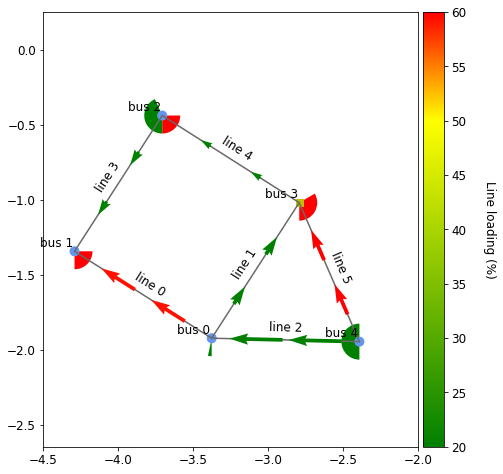
\includegraphics[width=0.5\columnwidth]{case_5.png}
\caption{The ``Case 5'' network on which the data is based, and an example visualization of the power flow.
  Line and bus IDs are indicated  the figure. The relative magnitude of the loads (red) and generators (green)
  are demonstrated using wedges surrounding each node. The magnitude of the current flowing in the line is
  demonstrated by the size of the arrows, and the color of the arrows indicates the line loading of each line.
}

\end{figure}

\subsection{Plot the data.}

\begin{enumerate}
\item Before beginning, make sure that your python environment is fully compatible by
  installing pandas, pytorch, matplotlib, and scikitlearn. You may e.g. need to use a downgraded
  version of Python.
\item Read in the data (hint: use \code{read\_csv} from pandas, which will create an object of
  type \code{pandas.DataFrame}). Determine the characteristics
  of the data: the columns, the time interval between data points, etc.
\item Using matplotlib (or some other package,) plot the active power of the loads and static
  generators (sgens). Comment on the characteristics of each of the loads and generators.

  \textbf{Hint}: It will be helpful to plot the data in different timescales (e.g. 1-2 weeks), instead of
  plotting the entire year. Plotting a rolling average of the results can also be helpful -- see
  \code{DataFrame.rolling(...).mean()} of pandas.
\item Plot the output data - the line loadings (in percent). Comment on any features.
\end{enumerate}

\subsection{Prepare the data.}

\begin{enumerate}
\item Split the DataFrame containing all data into an input (``x'') DataFrame (the load and generator
  power values) and an output (``y'') DataFrame (the line loadings of each line in the network).
\item Split the data into training and testing subsets. For this, you can use \code{train\_test\_split} from \code{sklearn.model\_selection}.
  A good rule of thumb is to reserve about 20\% of the dataset for testing. Comment on why randomizing the data may be important, versus simply
  splitting the sequential data points in two.
\item To prepare the data for input into the neural network, use a scaler
  (e.g. \code{StandardScaler} from the sklearn.preprocessing module) to force the data closer to
  the (0,1) range. \textbf{Remember to do this for both the input x and the output y data!}
\end{enumerate}

\subsection{Create and train a neural network.}

\begin{enumerate}
\item Create a simple neural network class, inheriting from \code{torch.nn.Module},
  as demonstrated in the lectures. The pytorch documentation and tutorials are also
  a good resource to help you.
  The network should have at least one hidden layer, and the
  size of the layers (input, hidden, output) should be modifiable.
\item Train the neural network, using the code snippets from the lecture as a guide. Recall
  that you need to define an optimizer and a loss function for this step. Plot the loss
  as a function of epoch during the model training step.
\end{enumerate}

\subsection{Test the neural network.}

\begin{enumerate}
\item Calculate the loss on the testing dataset that was set aside.
  \textbf{Remember that the inputs and outputs need to be transformed in the same way as in the training step!}
  Comment on the result.
\item For either the test dataset or the train dataset, calcluate and plot the {\textbf{absolute residual}}
  ($y_\mathrm{pred}-y_\mathrm{actual}$) and {\textbf{relative residual}} ($(y_\mathrm{pred}-y_\mathrm{actual})/y_\mathrm{actual}$)
  between the line loading that the model predicts and the ``true'' line loading calculated
  by the explicit power flow calculation. Do this for each line loading.\\[2mm]
  {\textbf{Note:}} to do this, you will need to transform the model output \code{y\_test\_pred} back to ``line loading'' units,
  which requires e.g. \code{y\_scaler.inverse\_transform(y\_test\_pred)}.
\end{enumerate}

\subsection{Optimize the neural network hyperparameters.}

\begin{enumerate}
\item In this case, the model hyperparameters are the number of hidden layers and the
  dimension (number of hidden nodes) per hidden layer. Try to determine the minimum number
  of layers/nodes required to solve this relatively simple grid problem. How many model parameters
  does this correspond to? (Hint: if your \code{model} inherits from \code{torch.nn.Module}, use
  \code{model.named\_parameters()} to see them explicitly).
\end{enumerate}

\section{Report}

The report is due within \textbf{14 days} after the date of the practical training. It must be
uploaded via the corresponding function in the virtual class room.\\

{\color{red}\textbf{Note: if you copy-pasted snippets of code from the internet, you must give
    proper credit by providing a link to the corresponding webpage.}}\\

The report consists of two parts:
\begin{itemize}
\item A completed python script, either in ``.ipynb'' or ``.py'' format.
  (If you use a Jupyter notebook, you can use the ``.ipynb'' file with annotated answers instead
  of the PDF document.)
  %% Please replace the extension with ``.txt'' before uploading.
\item A PDF document containing:
  \begin{itemize}
  \item Answers to the questions or prompts in Section~\ref{ml_pf}.
  \item The requested data and result plots. Be sure to properly label axes and data.
  \item This exercise was a demonstration of supervised learning, i.e. where a power flow
    solver was run to find the ``true'' result. How can this machine problem -- i.e. the problem
    of solving the power flow equations -- be reformulated
    as an \textbf{unsupervised learning problem}, i.e. without the benefit of having labeled
    data available (i.e. without a separate power flow solver at hand)?
  \item Thinking about appraches for more complicated grid networks, what ANN architectures
    might be appropriate for leveraging the structure inherent to the grid data?
  \end{itemize}
\end{itemize}

\section{Useful code snippets}

Here is a code snippet for plotting multiple data columns in a DataFrame:

\begin{verbatim}
import matplotlib.pyplot as plt
fig,ax = plt.subplots(1,1,figsize=(10,8))
columns = ['A','B','C'] # column names to plot
ax.plot(the_dataframe[columns],label=columns)
ax.set(xlabel='x label',ylabel='y label')
ax.legend()
\end{verbatim}

To restrict the range of a DataFrame (e.g. from timestep 5 to timestep 20), for instance
to plot certain time ranges:

\begin{verbatim}
data[5:20]
\end{verbatim}

If you encounter the error ``Error: Argument must be tensor, not ...'' for a given variable
$z$, then the solution is to wrap $z$ according to the following:

\begin{verbatim}
torch.tensor(z).float()
\end{verbatim}

To import e.g. the Adam Optimizer in Torch:

\begin{verbatim}
from torch.optim import Adam
\end{verbatim}


\end{document}
